\documentclass[class=report,crop=false, 12pt]{standalone}
\usepackage[screen,nosolutions]{../scratch}

\begin{document}

\titre[S]{Répéter}
%===============================

\insertvideo{iWEGE7JnVAI}{Répéter -- Activité 1}

\insertvideo{DfXBBizL1YE}{Répéter -- Activité 2}

\insertvideo{VddWNA1gNP8}{Répéter -- Activité 3}

\bigskip
\bigskip


\begin{activite}
Trace un escalier, comme sur cette figure. À chaque marche, Scratch monte de 10 puis avance de 20.

\begin{center}
  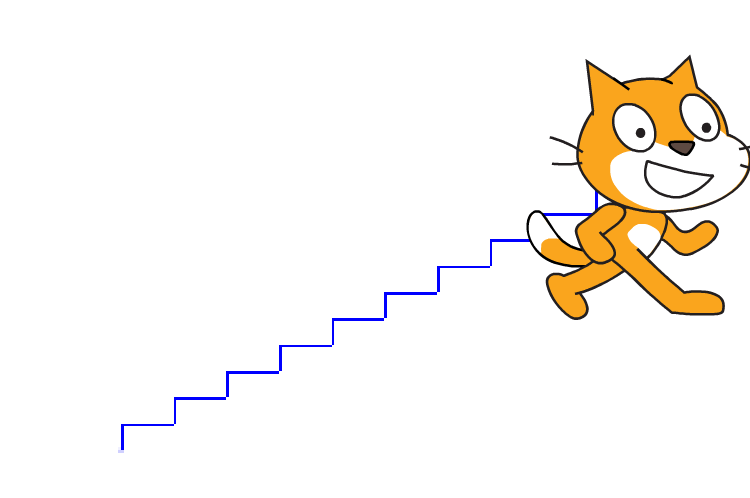
\includegraphics[scale=\scaleecran]{ecran-02-ex1}   
\end{center}

\textbf{Blocs utiles.}
\begin{itemize}
  \item Le bloc le plus utile sera le bloc répéter 10 fois. Toutes les instructions placées à l'intérieur de ce bloc seront répétées 10 fois.
  
\begin{center}
  
\includegraphics[scale=\scalebloc,scale=1.3]{bloc-02-ex1}
\end{center} 
  
  \item Autres blocs déjà vus : s’orienter à 0\textdegree\ (vers le haut), s’orienter à 90\textdegree\ (vers la droite)...
Et aussi aller à $x=0$, $y = 0$, effacer tout, stylo en position d’écriture, attendre 1 seconde...
\end{itemize}

\end{activite}


\begin{activite}
Trace un polygone comme sur la figure suivante. Change de couleur à chaque côté. 
\begin{center}
  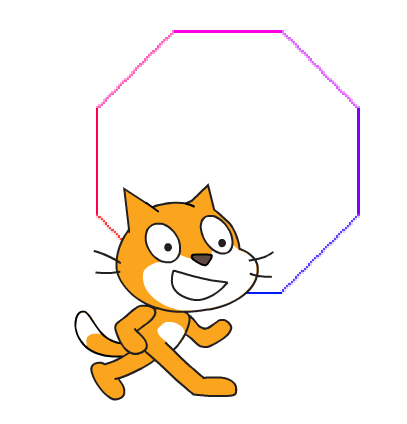
\includegraphics[scale=\scaleecran]{ecran-02-ex2}   
\end{center}


\textbf{Blocs utiles.}
\begin{itemize}
  \item Tourner à gauche de 45 degrés
  \item Ajouter 10 à la couleur du stylo
\end{itemize}
\end{activite}


\begin{activite}
Trace des escaliers comme sur la figure.
\begin{center}
  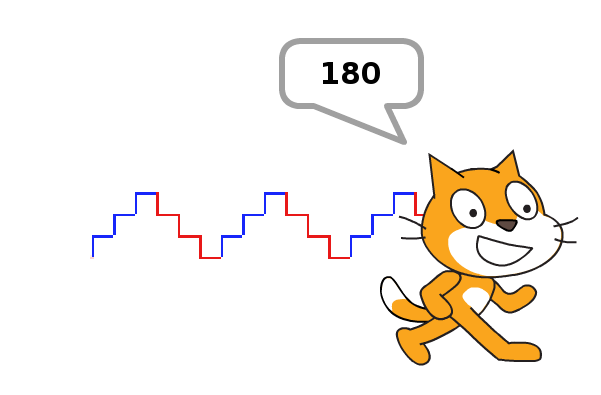
\includegraphics[scale=\scaleecran]{ecran-02-ex3}   
\end{center}

\begin{itemize}
  \item On répète trois fois : le chat monte de 10 puis avance de  10 (escalier bleu).
  \item On répète trois fois  : le chat descend de 10 puis avance de  10  (escalier rouge).
  \item On répète ces deux opérations trois fois.
  \item De plus, tu peux changer la couleur du trait et afficher la valeur de l'abscisse $x$ de Scratch lorsqu'il s'arrête.
\end{itemize}
\end{activite}

\ifx \displaysolutions \myzero
\else
\begin{code}
\onesolution{Répéter}{Activité 1}{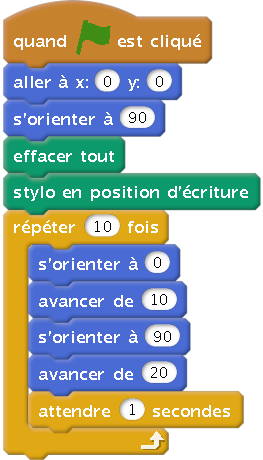
\includegraphics[scale=\scalesolution]{code-02-ex1}}
\onesolution{Répéter}{Activité 2}{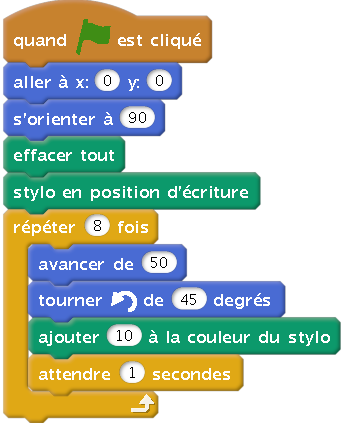
\includegraphics[scale=\scalesolution]{code-02-ex2}}
\onesolution{Répéter}{Activité 3}{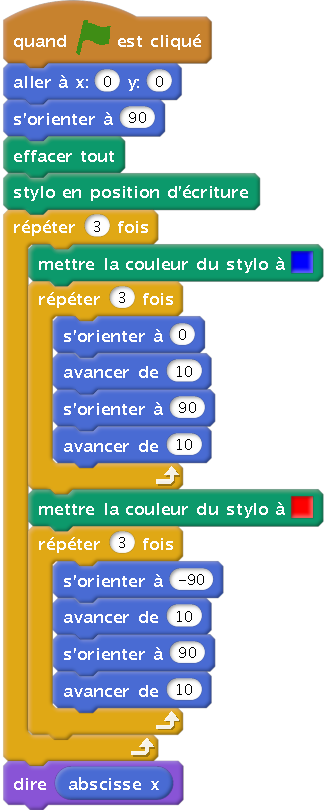
\includegraphics[scale=\scalesolution]{code-02-ex3}}    
\end{code}
\fi

\end{document}

